\chapter{Multilingual machine translation}
\label{chapter12}
\setcounter{enums}{0}


\noindent Using information structure can improve multilingual machine
translation.  A machine translation system informed by information
structure is capable of reducing the number of infelicitous
translations dramatically. This reduction has two effects on the
performance of \isi{transfer-based} machine translation
\citep{song:bender:11}: First, the processing burden of the machine
translation component which ranks the translations and selects only
suitable results can be greatly lightened, which should improve
translation speed.  Second, although it is still necessary to employ a
re-ranking model for choosing translations, we can start from a
refined set of translations, which should improve translation
accuracy.


Section \ref{2:sec:tmt} goes over the basis of transfer-based machine
translation.  Section \ref{12:sec:machinery} offers an explanation of
how \isi{ICONS} (Individual CONStraints)\is{Individual CONStraints}
operate in \isi{transfer-based} machine translation. Section
\ref{12:sec:processor} addresses the processor the current work
employs for testing machine translation. Section
\ref{13:sec:evaluation} conducts an evaluation to examine how many
infelicitous translations are filtered out by means of ICONS.



\section{Transfer-based machine translation}
\label{2:sec:tmt}


The basic method I employ for testing machine translation herein is
built on the symbolic approach to machine translation, which normally
consists of three stages:\is{transfer-based}\is{generation} (i)
parsing, (ii) transfer, and (iii) generation.  Since MRS is not an
interlingua\is{MRS} (a meaning representation language in which the
representations are identical for all languages), using MRS for
machine translation requires an independent stage to convert one MRS
into another MRS. This stage is called transfer, and is carried out
between parsing and generation.  \is{transfer-based}\is{generation}




Figure~\ref{fig:mt}, adapted from \citet{oepen:etal:07} and
\citet{song:etal:10},\is{MRS} is illustrative of the MRS-based
architecture of machine translation. The first step (i.e.\ parsing)
analyses a sentence with a computational grammar for the source
language, whose output is a form of semantic representation such as a
(near) logical form.  The output of the first step serves as the
source of the next step (i.e.\ transfer), which is called MRS$_s$
(i.e.\ an input MRS).  The transfer module converts the source
representation obtained from the parsing process into another type of
representation compatible with the target language, which is called
MRS$_t$ (i.e.\ an output MRS).  MRS$_t$ is used as the source for the
final step (i.e.\ generation), which constructs one or more surface
forms built from the semantic representation. As a consequence, the
two surface forms in the source language and the target language are
compatible with a common meaning representation.





\begin{figure}[!t]
\begin{center} 
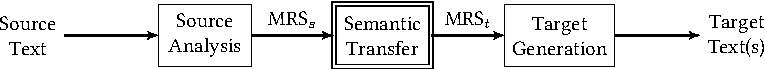
\includegraphics[width=.9\textwidth]{pdf/mt.pdf}
\caption{HPSG/MRS-based MT architecture}
\label{fig:mt}
\end{center}
\end{figure}


\section{Basic machinery}
\label{12:sec:machinery}

A graph presented in (\ref{fig:mmt:basic}a) represents an \ili{English}
sentence in which the subject \textit{the \textsc{dog}} bears the
A-accent, thereby plays the role of \tdl{semantic-focus}.\is{semantic focus}
The second graph in (\ref{fig:mmt:basic}b) represents the \ili{Japanese}
translation, in which the subject \textit{inu} `dog' is combined with
the nominative marker \ga that signals \tdl{non-topic}.  That is to
say, although the two sentences provided in (\ref{fig:mmt:basic}a--b)
are proper translations of each other, information is differently
structured.

\myexe{\enumsentence{\toplabel{fig:mmt:basic}
\begin{tabular}[t]{lllll}
a. & \evnup{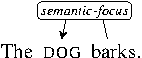
\includegraphics{pdf/basic1-eng.pdf}} & \xspace &
b. & \evnup{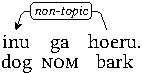
\includegraphics{pdf/basic1-jpn.pdf}} \\
\end{tabular}}}



\noindent Note that \tdl{non-topic} is a supertype of
\tdl{semantic-focus} in the type hierarchy of \tdl{info-str} given in
Figure~\ref{fig:info-str}
\mypage{fig:info-str}.\is{\textit{info-str}}\is{semantic focus}  
This ability to partially specify information
structure allows us to reduce the range of outputs in translation
while still capturing all legitimate possibilities.



Two hypothetical suffixes \textit{-a} and \textit{-b} are employed for testing
hereafter, and they represent the A and B accents in \ili{English}
\citep{bolinger:61,jackendoff:72} respectively.  Note that the \textit{-b}
suffix cannot be attached to the verb \textit{barks}, because verbs
presumably cannot be marked via B-accent for the information
structure role of \tdl{topic} in English.\is{topic}  \textit{The dog barks}
without any information structure marking logically can be interpreted
as six types of sentences (3\ensuremath{\times}2).\is{A-accent}\is{B-accent}




\myexe{\enumsentence{\label{exe:eng}
\begin{tabular}[t]{ll}
dog & dog: [ ICONS: \ensuremath{<} \ensuremath{>} ] \\
    & dog-a: [ ICONS: \ensuremath{<} e2 \textbf{semantic-focus} x4 \ensuremath{>} ]\\
    & dog-b: [ ICONS: \ensuremath{<} e2 \textbf{contrast-or-topic} x4 \ensuremath{>} ]\\
bark &  barks: [ ICONS: \ensuremath{<} \ensuremath{>} ] \\
    & barks-a: [ ICONS: \ensuremath{<} e2 \textbf{semantic-focus} e2 \ensuremath{>} ]
\end{tabular}}}


\noindent However, if we apply \isi{ICONS} to generation, we can
filter out sentences which are not equivalent to the input sentence
with respect to information structure. For example, if the input
sentences are \textit{The \textsc{dog} barks} and \textit{The
  \textbf{dog} barks} in which the subject bears the A and B accents
respectively, they can be monolingually paraphrased as
(\ref{exe:para:eng}). That is, four infelicitous sentences from each
set of sentences can be removed.  Two sentences in
(\ref{exe:para:eng}a-i) and (\ref{exe:para:eng}a-iii) cannot be
generated because the subject does not include any value in ICONS. In
other words, information structure-marked constituents in the source
cannot be generated as an unmarked constituent in the target.  Two
sentences in (\ref{exe:para:eng}a-v) and (\ref{exe:para:eng}a-vi)
cannot be generated, either.\is{B-accent} This is because the
B-accented subject conveys \tdl{contrast-or-topic} which is
incompatible with \tdl{semantic-focus}.\is{semantic focus}\is{contrastive focus}
The same goes for (\ref{exe:para:eng}b): Since only the last two sentences are
compatible with the information structure meaning that the input
sentence conveys, the others cannot be paraphrased with respect to
information structure.





\myexe{\enumsentence{\label{exe:para:eng}
\begin{tabular}[t]{ll}
a. & The dog-\textbf{a} barks [ ICONS: \ensuremath{<} e2 \textbf{semantic-focus} x4 \ensuremath{>} ]\\
 & \xtab(i) \Midline{The dog barks}\\
 & \xtab(ii) The dog-a barks\\
 & \xtab(iii) \Midline{The dog barks-a}\\
 & \xtab(iv) The dog-a barks-a\\
 & \xtab(v) \Midline{The dog-b barks}\\
 & \xtab(vi) \Midline{The dog-b barks-a}\\
\end{tabular}}}

\myexe{\enumsentence[]{
\begin{tabular}[t]{ll}
b. & The dog-\textbf{b} barks [ ICONS: \ensuremath{<} e2 \textbf{contrast-or-topic} x4 \ensuremath{>} ]\\
 & \xtab(i) \Midline{The dog barks}\\
 & \xtab(ii) \Midline{The dog-a barks}\\
 & \xtab(iii) \Midline{The dog barks-a}\\
 & \xtab(iv) \Midline{The dog-a barks-a}\\
 & \xtab(v) The dog-b barks\\
 & \xtab(vi) The dog-b barks-a\\
\end{tabular}}}


\noindent The same goes for Japanese in which lexical markers signal
information structure.\is{lexical markers} There are at least three
Japanese translations (i.e.\ case-marking, \wa-marking, and
null-marking) corresponding to \textit{The dog barks}, but case-marked
NPs cannot be paraphrased into \wa-marked NPs within our
\tdl{info-str} hierarchy given in
Figure~\ref{fig:info-str},\is{\textit{info-str}} and vice versa. Note
that null-marked items in Japanese (e.g.\ \textit{inu} in
\ref{exe:para:jpn}a-iii and \ref{exe:para:jpn}b-iii) are assigned
\tdl{non-focus} \citep{yatabe:99}, which is compatible with both
\tdl{non-topic} in (\ref{exe:para:jpn}a) and \tdl{contrast-or-topic}
(\ref{exe:para:jpn}b). Thus, both \textit{inu ga hoeru} and
\textit{inu wa hoeru} can be paraphrased into \textit{inu hoeru}.





\myexe{\enumsentence{\label{exe:para:jpn}
\begin{tabular}[t]{ll}
a. & inu \textbf{ga} hoeru [ ICONS: \ensuremath{<} e2 \textbf{non-topic} x4 \ensuremath{>} ]\\
 & \xtab(i) inu ga hoeru\\
 & \xtab(ii) \Midline{inu wa hoeru}\\
 & \xtab(iii) inu hoeru\\
b. & inu \textbf{wa} hoeru [ ICONS: \ensuremath{<} e2 \textbf{contrast-or-topic} x4 \ensuremath{>} ]\\
 & \xtab(i) \Midline{inu ga hoeru}\\
 & \xtab(ii) inu wa hoeru\\
 & \xtab(iii) inu hoeru\\
\end{tabular}}}


Translating across languages is constrained in the same manner. An
\ili{English} sentence (\ref{exe:tran}a) cannot be translated into
(\ref{exe:tran}a-ii) and (\ref{exe:tran}a-iii), because the
\tdl{semantic-focus} role that \textsc{dog} involves is incompatible
with the \tdl{contrast-or-topic} role that \textit{wa} assigns and the
\tdl{non-focus} role that the null marker (indicated by \ensuremath{\emptyset})
involves. On the other hand, a Japanese sentence (\ref{exe:tran}b) can
be translated into only (\ref{exe:tran}b-ii) and
(\ref{exe:tran}b-iv). First, because \tdl{non-topic}, which comes from
the nominative marker \textit{ga},\is{B-accent} is contradictory to
\tdl{contrast-or-topic} that the B-accent signals in English,
(\ref{exe:tran}b-v) and (\ref{exe:tran}b-vi) are filtered out.
Second, because the constituent corresponding to the \ga-marked
subject should introduce an \tdl{info-str} element into ICONS,
(\ref{exe:tran}b-i) and (\ref{exe:tran}b-iii) are ruled out.



\myexe{\enumsentence{\label{exe:tran}
\begin{tabular}[t]{ll}
a. & The dog-\textbf{a} barks [ ICONS: \ensuremath{<} e2 \textbf{semantic-focus} x4 \ensuremath{>} ]\\
 & \xtab(i) inu ga hoeru\\
 & \xtab(ii) \Midline{inu wa hoeru}\\
 & \xtab(iii) \Midline{inu hoeru}\\
b. & inu \textbf{ga} hoeru [ ICONS: \ensuremath{<} e2 \textbf{non-topic} x4 \ensuremath{>} ]\\
 & \xtab(i) \Midline{The dog barks}\\
 & \xtab(ii) The dog-a barks\\
 & \xtab(iii) \Midline{The dog barks-a}\\
 & \xtab(iv) The dog-a barks-a\\
 & \xtab(v) \Midline{The dog-b barks}\\
 & \xtab(vi) \Midline{The dog-b barks-a}\\
\end{tabular}}}




\section{Processor}
\label{12:sec:processor}

The processor the present work uses for the purpose of evaluation is
\isi{\ace}.\footnote{\isi{\ace}
  (\myurl{http://sweaglesw.org/linguistics/ace}) is the first
  \isi{DELPH-IN} processor to specifically handle \isi{ICONS} as part
  of the MRS, and then \isi{\agree}~(\citealt{slayden:12}) also uses
  \isi{ICONS} for constraining information structure in parsing and
  generation.}  \isi{\ace} parses the sentences of natural languages,
and generates sentences based on the MRS\is{MRS} (Minimal Recursion
Semantics, \citealt{copestake:etal:05}) representation that the parser
creates.  As the data \isi{\ace} uses \isi{DELPH-IN} grammars,
including \lingo \isi{Grammar Matrix} grammars created by the
customization system
\citep{bender:flickinger:05,drellishak:09,bender:etal:10} and resource
grammars (e.g.\ the ERG (English Resource Grammar,
\citealt{flickinger:00}).






When creating the data file of \isi{\ace}, \ace refers to parameters
described in \textit{ace/config.tdl}. In the configuration file,
grammar users can choose whether or not \isi{ICONS} is used in MRS
representation. The snippet that enables \isi{ICONS} to be included in MRS
representation is as follows.

\myexe{\enumsentence{\toplabel{tdl:config}
\evnup{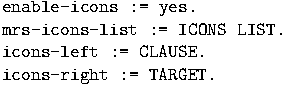
\includegraphics{pdf/tdl-config.pdf}}}}


\isi{\ace} carries out ICONS-based generation via subsumption check,
using the type hierarchy \tdl{info-str} (presented in
Figure~\ref{fig:info-str}).\is{\textit{info-str}} \isi{\ace} generates
all potential sentences that logically fit in the input MRS not
considering the constraints on \isi{ICONS} beforehand. After that, if
the data file of the grammar for generation is compiled with the
parameters given in \myref{tdl:config}, \isi{\ace} starts
postprocessing the intermediate results.  Depending on the subsumption
relationship of information structure meanings, sentences mismatching
the values in the \isi{ICONS} list are filtered out in this step.  For
example, if \tdl{semantic-focus} is assigned to a specific individual
in the source MRS,\is{MRS} only outputs that provide an \isi{ICONS}
element for that individual can be produced.\is{\textit{info-str}} The
\tdl{info-str} value an individual has in the output should be the
same as that in the input (i.e.\ \tdl{semantic-focus})\is{semantic
  focus} or its supertypes (e.g.\ \tdl{focus}, \tdl{non-topic},
etc.). For instance, an A-accented constituent in \ili{English}
(e.g.\ \textsc{dog}) contributes an \isi{ICONS} element whose value is
\tdl{semantic-focus}, and this element is translated as a \ga-marked
constituent (e.g.\ \textit{inu ga}) whose value is monolingually
\tdl{non-topic} in \ili{Japanese}. Note that \tdl{non-topic} subsumes
\tdl{semantic-focus} in the type hierarchy presented in
Figure~\ref{fig:info-str}.\is{\textit{info-str}} A completely
underspecified output for each \isi{ICONS} element is not acceptable
in generation.\is{underspecification} For instance, an A-accented
\textsc{dog} that introduces an \isi{ICONS} element cannot be
paraphrased as an unaccented \textit{dog} that does not contribute any
\isi{ICONS} element.\is{A-accent} By contrast, the opposite direction
is acceptable.  If a constituent introduces no \isi{ICONS} element in
the input, the output can include an information-structure marked
constituent. For instance, an unaccented \textit{dog} can be
paraphrased as an A-accented \textsc{dog} in generation.






\section{Evaluation}
\label{13:sec:evaluation}


\subsection{Illustrative grammars}
\label{13:ssec:grammars}

In order to verify a linguistic hypothesis with reference to a
computational grammar,\is{illustrative grammars} it is a good strategy
to use a compact grammar presenting the fundamental rules in a precise
manner. Illustrative grammars are constructed for this purpose.  The
illustrative languages used here are \ili{English}, \ili{Japanese},
and \ili{Korean}.  These languages are chosen, because the resource
grammars for each of the language will be the main concern in my
further study.\footnote{The computational grammars include \isi{ERG}
  \citealp{flickinger:00}, \isi{Jacy} \citep{siegel:etal:16}, and
  \isi{KRG} \citep{kim:etal:11}.}  The information structure
properties each language has are summarized in the following
subsections.



\subsubsection{English}
\label{13:sssec:eng}


As is well known,\is{prosody} \ili{English} employs prosody for
expressing information structure.  Without consideration of the
prosodic patterns, we could not draw the basic picture of
information-structure related phenomena in English.\footnote{English
  also makes use of some constructional means to configure focus and
  \isi{topic}. These include \isi{focus}/topic \isi{fronting},
  \isi{clefting}, etc. Nonetheless, these have to do with various
  grammatical components. For example, implementing grammatical
  modules for cleft constructions necessitates many \isi{TDL}
  statements for relative clauses as an essential
  prerequisite.\is{relative clause} This involves too much complexity
  for an illustrative grammar to cover.  For this reason, the
  illustrative grammar for English in this evaluation is exclusively
  concerned with prosody.} There are quite a few previous studies on
how prosody is realized with respect to information structure
\citep{jackendoff:72,steedman:00,kadmon:01,buring:03,hedberg:06}, but
there seems to be no clear consensus (as surveyed earlier in Section
\ref{4:sec:prosody}).\is{illustrative grammars} The illustrative
grammar for English makes use of just the traditional distinction of
the A and B accents \citep{bolinger:58}. In order to articulate them
as a string for ease of exposition, the two hypothetical suffixes
\textit{-a} and \textit{-b} are used. However, the meanings that the
accents take charge of are represented differently from the
traditional approach. The information structure meanings that
\textit{-a} and \textit{-b} convey are marked following
\citeauthor{hedberg:06}'s argument: \textit{-a} for
\tdl{semantic-focus} and \textit{-b} for
\tdl{contrast-or-topic}.\is{semantic focus} The AVMs are already
presented in Section \ref{9:ssec:eng} \mypage{avm:fc:tp:eng}.



\subsubsection{Korean}
\label{13:ssec:kor}


The illustrative grammar for \ili{Korean} includes two kinds of
grammatical sets of constraints for expressing information
structure.\is{lexical markers} The first one employs lexical markers,
such as \ika and \lul for case marking, \nun for \isi{topic} marking,
and \ensuremath{\emptyset}~for null marking. The AVMs for these
markers are presented in Section
\ref{9:ssec:jpn:kor} \mypage{avm:ika:nun:kor}.  The second fragment
aims to handle scrambling. The AVMs for constraining scrambling
constructions are provided in Section
\ref{10:sec:scrambling} \mypage{avm:top:scr}.\is{scrambling} These
AVMs use different rules instantiating \tdl{head-subj-phrase} and
\tdl{head-comp-phrase} with reference to lexical markings of daughters
(i.e.\ MKG).\is{MKG}


\subsubsection{Japanese}
\label{13:ssec:jpn}



As mentioned before,\is{HPSG} the present study respects the
traditional ways of dealing with lexical markers in \ili{Japanese} and
\ili{Korean} from different points of view. While lexical markers in
Korean are dealt with as suffixes \citep{kim:yang:04}, those in
Japanese are treated as adpositions
\citep{siegel:99}.\is{adposition}\is{illustrative grammars} Other than
this difference, the illustrative grammar for Japanese has the same
configuration as that for Korean explained above. Notably, the null
marker in Japanese is constrained by a lexical rule in the current
work \mypage{avm:ga:wa:jpn}, which is different from previous
HPSG-based suggestion about so-called case-ellipsis
\citep{yatabe:99,sato:tam:12}.




\subsection{Testsuites}
\label{13:ssec:testsuites}


The \isi{testsuites} (a collection of sentence to be modeled) for this
multilingual machine translation testing are provided in
(\ref{exe:testsuite:eng}-\ref{exe:testsuite:kor}); \ili{English},
\ili{Japanese}, and \ili{Korean}, respectively.  There is one
intransitive sentence and one transitive sentence in English, and they
are encoded with two hypothetical suffixes and differentiated as
allosentences.



\myexe{\enumsentence{\label{exe:testsuite:eng}
\evnup{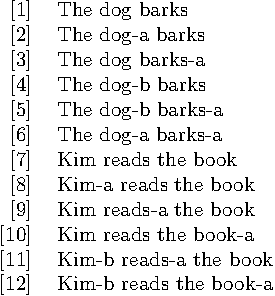
\includegraphics[scale=0.9]{pdf/item-eng.pdf}}}}

\myexe{\enumsentence{\label{exe:testsuite:jpn}
\evnup{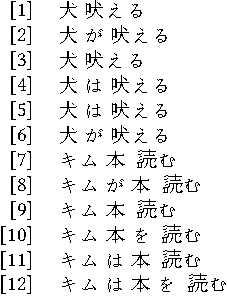
\includegraphics[scale=0.9]{pdf/item-jpn.pdf}}}}

\myexe{\enumsentence{\label{exe:testsuite:kor}
\evnup{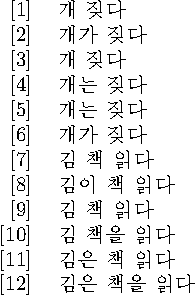
\includegraphics[scale=0.9]{pdf/item-kor.pdf}}}}



\subsection{An experiment}
\label{12:ssec:experiments}


\begin{table}[!t]
\small
\centering
\begin{tabular}{ccc}
Table 13.1: \# of outputs without \isi{ICONS} & \mbox{ } &
Table 13.2: \# of outputs with ICONS\\ 
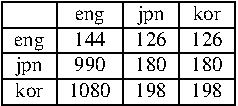
\includegraphics{pdf/tbl_total-number-of-output2.pdf} & & 
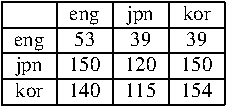
\includegraphics{pdf/tbl_total-number-of-output.pdf} \\
\end{tabular}
\end{table}


\begin{figure}[!t]
\begin{center} 
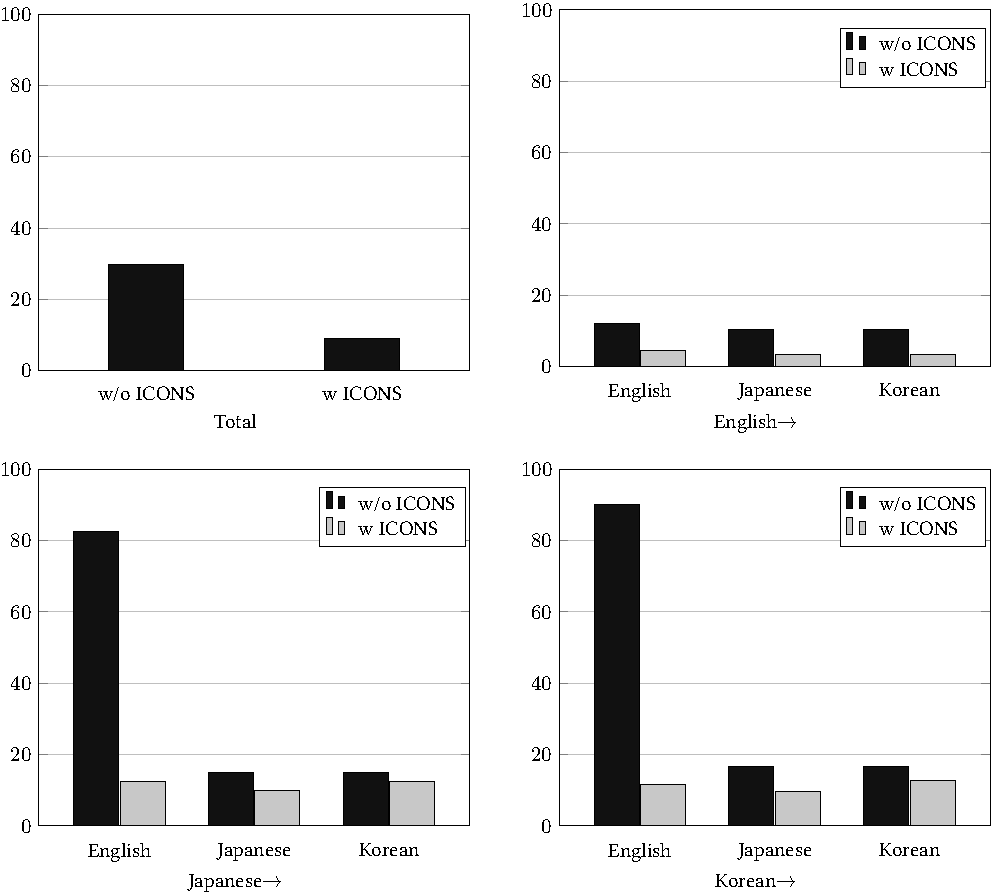
\includegraphics[width=.9\textwidth]{pdf/comparison2.pdf}
\caption{Average \# of outputs}
\label{fig:comp:mmt}
\end{center}
\end{figure}


\noindent All test items presented in \myref{exe:testsuite:eng} and
their translations in \ili{Japanese} and \ili{Korean} are parsed,
transferred, and generated.\is{transfer-based}\is{generation}  Table 13.1 and Table 13.2 show the number
of translation results in each translation pair. The first column in
each table indicates the source language, and the first row indicates
the target language. For example, [English \ensuremath{\rightarrow}
Japanese] produces 126 translations when not using ICONS, and 39
translations when using ICONS.\is{testsuites}


As indicated in the tables, the number of generated sentences
dramatically decreases when using ICONS. The total number of
translation outputs in Table 15.1 is 3,222, while that in Table 15.2
is merely 960.\footnote{When the source language is not \ili{English} and
  the target language is English, the numbers are rather big in Table
  15.1. This is because English employs number and COG-ST features,
  while \ili{Japanese} and \ili{Korean} do not. For example,
  \textit{inu} in Japanese can be translated into at least four NP
  types in English: \textit{a dog}, \textit{the dog}, \textit{the
    dogs}, and \textit{dogs}.} That means approximately 70\% of the
translations are filtered out in total when using ICONS.



The four charts in Figure~\ref{fig:comp:mmt} compare the average
number of outputs in total and in each translation pair. The decrease
indicated in each bar chart shows that information structure can be
used to filter out inappropriate sentences from the translation
result.




These charts show that when translating \ili{Japanese} and
\ili{Korean} to \ili{English} many outputs are filtered out. The main reason
for the dramatic decrease in [Japanese \ensuremath{\rightarrow} English]
and [Korean \ensuremath{\rightarrow} English] is that the illustrative
grammar for English includes a lexical rule to mark \isi{focus} on verbal
items, while the illustrative grammars for Japanese and Korean do
not.\is{illustrative grammars} When a verb is focused in the English grammar, 
the lexical rule introduces a \tdl{focus} element into ICONS.\is{\textit{info-str}}
In contrast, verbs cannot involve any \tdl{info-str} 
value in the current illustrative grammars
for Japanese and Korean. Thus, the huge difference in [Japanese
\ensuremath{\rightarrow} English] and [Korean \ensuremath{\rightarrow}
English] is largely caused by the different marking system for verbal
items.


Finally, I verified 108 sets of translation outputs (9 directions
\ensuremath{\times} 12 test items) by hand. The same problem was also
found. When an \ili{English} item includes an A-accented verb
(e.g.\ \textit{barks-a} and \textit{reads-a}),\is{A-accent} the item
cannot be translated into \ili{Japanese} and \ili{Korean}. This
suggest that there might be a problem with the strategy of requiring
some information structure marking in the output for an item if there
is some in the input.  Other than this difference, the translation
outputs were legitimate and felicitous.  I also sampled the filtered
translations to verify that they were all infelicitous ones, and found
that this information structure-based model works for them, too.




\section{Summary}
\label{13:sec:sum}

It is my firm opinion that translating should mean reshaping the ways
in which information is conveyed, not simply changing words and
reordering phrases.  In almost all human languages, articulation of
sentential constituents is conditioned by information
structure. Because the means of expressing information structure
differs across languages, identifying how information is structured in
a given set of languages plays a key role in achieving felicity in a
machine translation between them.\is{felicity} Hence, information
structure is of great help to multilingual machine translation in that
information structure facilitates more felicitous translations.  This
chapter conducted a small experiment to support this
hypothesis.\is{illustrative grammars} I created three illustrative
grammars for \ili{English}, \ili{Japanese}, and \ili{Korean} following my
ICONS-based analyses presented thus far. In the test of transfer-based
machine translation,\is{transfer-based} I found that using information
structure served to filter out infelicitous translations
dramatically. This testing should be further elaborated in future work
using resource grammars, such as the \isi{ERG}
(\citealt{flickinger:00}), \isi{Jacy} (\citealt{siegel:etal:16}),
and the \isi{KRG} (\citealt{kim:etal:11}).


